\section{Introduction}

\subsection{}

\begin{frame}
    \frametitle{Resources}

    \begin{itemize}
        \item Ian Goodfellow, Yoshua Bengio, and Aaron Courville.
        \emph{Deep Learning}.
        MIT Press, 2016
        \nocite{GoodfellowDL}
        \begin{itemize}
            \item Excellent primer
            \item \blueurl{http://www.deeplearningbook.org}
        \end{itemize}
        \item These slides: \blueurl{https://goo.gl/DqARo4}
        \item References at the end of these slides
        \item Physics-specific resources
        \begin{itemize}
            \item Search \texttt{https://meetings.aps.org/Meeting/DFD1x/} \texttt{SearchAbstract} (with \texttt{x} = 7, 6, etc.) for ML abstracts
            \item NIPS 2017 Workshop on \bluelink{https://dl4physicalsciences.github.io}{Deep Learning for Physical Sciences}
        \end{itemize}
        \item Talk to me! \smiley
    \end{itemize}
\end{frame}

\begin{frame}
    \frametitle{A super brief history of machine learning}
    \begin{itemize}
        \item Mid-20th century: birth of essential machine learning ideas
        \item 1957: Birth of the \alert{perceptron}, basis of modern neural networks \citep{RosenblattCornell57}
        \item 1970s--1980s: discovery of \alert{backpropagation} to train ML models efficiently \citep{RumelhartNature86}
        \item 1980s: \alert{convolutional} neural networks, \alert{recurrent} neural networks, \alert{reinforcement} learning
        \item 1989: \alert{Universal approximation theorem}: neural networks can model anything nice \citep{CybenkoMCSS89,HornikNN89}
    \end{itemize}
    \pause

    So why haven't we heard much about ML until recently?
    \begin{itemize}
        \item 1970s--1990s: \alert{AI Winter}: ML thought to be intractable and unsexy.
        Rejected by much of the scientific community as useless!
    \end{itemize}
    \pause

    What changed?
    \begin{itemize}
        \item 2010s: emergence of \alert{deep learning} coupled with \alert{big data} $\implies$ ML starts to achieve the impossible
    \end{itemize}
\end{frame}

\begin{frame}
    \frametitle{Machine learning in fluid dynamics?}
    \# APS DFD abstracts with ``machine learning,'' ``neural network,'' or ``deep learning''

    \begin{center}
        \begin{tabular}{r|cccc}
            year & 2014 & 2015 & 2016 & 2018 \\
            \hline
            \# & 8 & 11 & 11 & \alert{28}
        \end{tabular}
    \end{center}
    \pause

    My perspective:

    \begin{itemize}
        \item Fluid dynamics is light years behind stats/CS in ML
        \item ML may or may not lead to a breakthrough in fluids modeling
        \begin{itemize}
            \item ML knowledge is developing at an astronomical rate
            \item The new norm: things thought impossible 10 years ago are now mundane
            \item But: ML doesn't inherently know physics.
            Should we expect ML to beat physics-based models?
            I don't know!
        \end{itemize}
    \end{itemize}
\end{frame}

\begin{frame}
    \frametitle{NIPS 2017: Deep Learning for Physical Sciences (1/4)}
    \bluelink{%
        https://dl4physicalsciences.github.io/files/nips_dlps_2017_slides_henrion.pdf%
    }{%
        Neural Message Passing for Jet Physics%
    } \citep{HenrionNIPS17} \\[1ex]

    \centering
    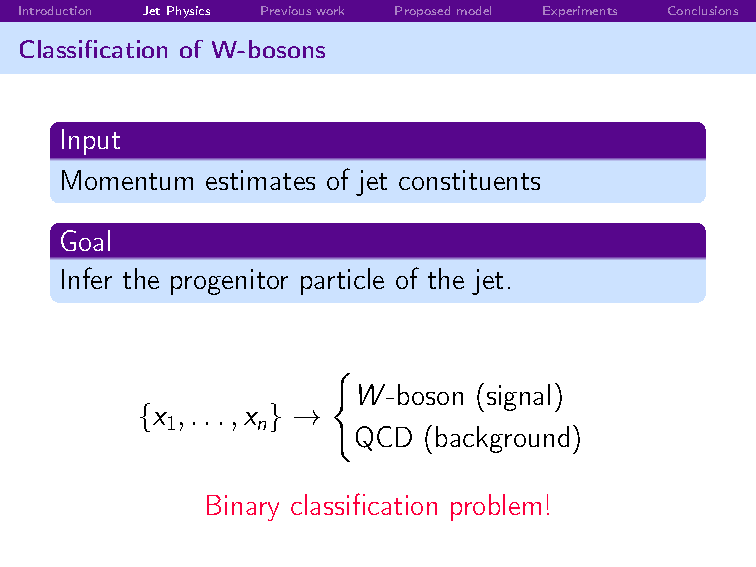
\includegraphics[width=0.86\textwidth]{boson}
\end{frame}

\begin{frame}
    \frametitle{NIPS 2017: Deep Learning for Physical Sciences (2/4)}
    \bluelink{%
        https://dl4physicalsciences.github.io/files/nips_dlps_2017_slides_welling.pdf%
    }{%
        Unrolling Inference: For Astronomy and MRI Imaging%
    } \citep{WellingNIPS17} \\[1ex]

    \centering
    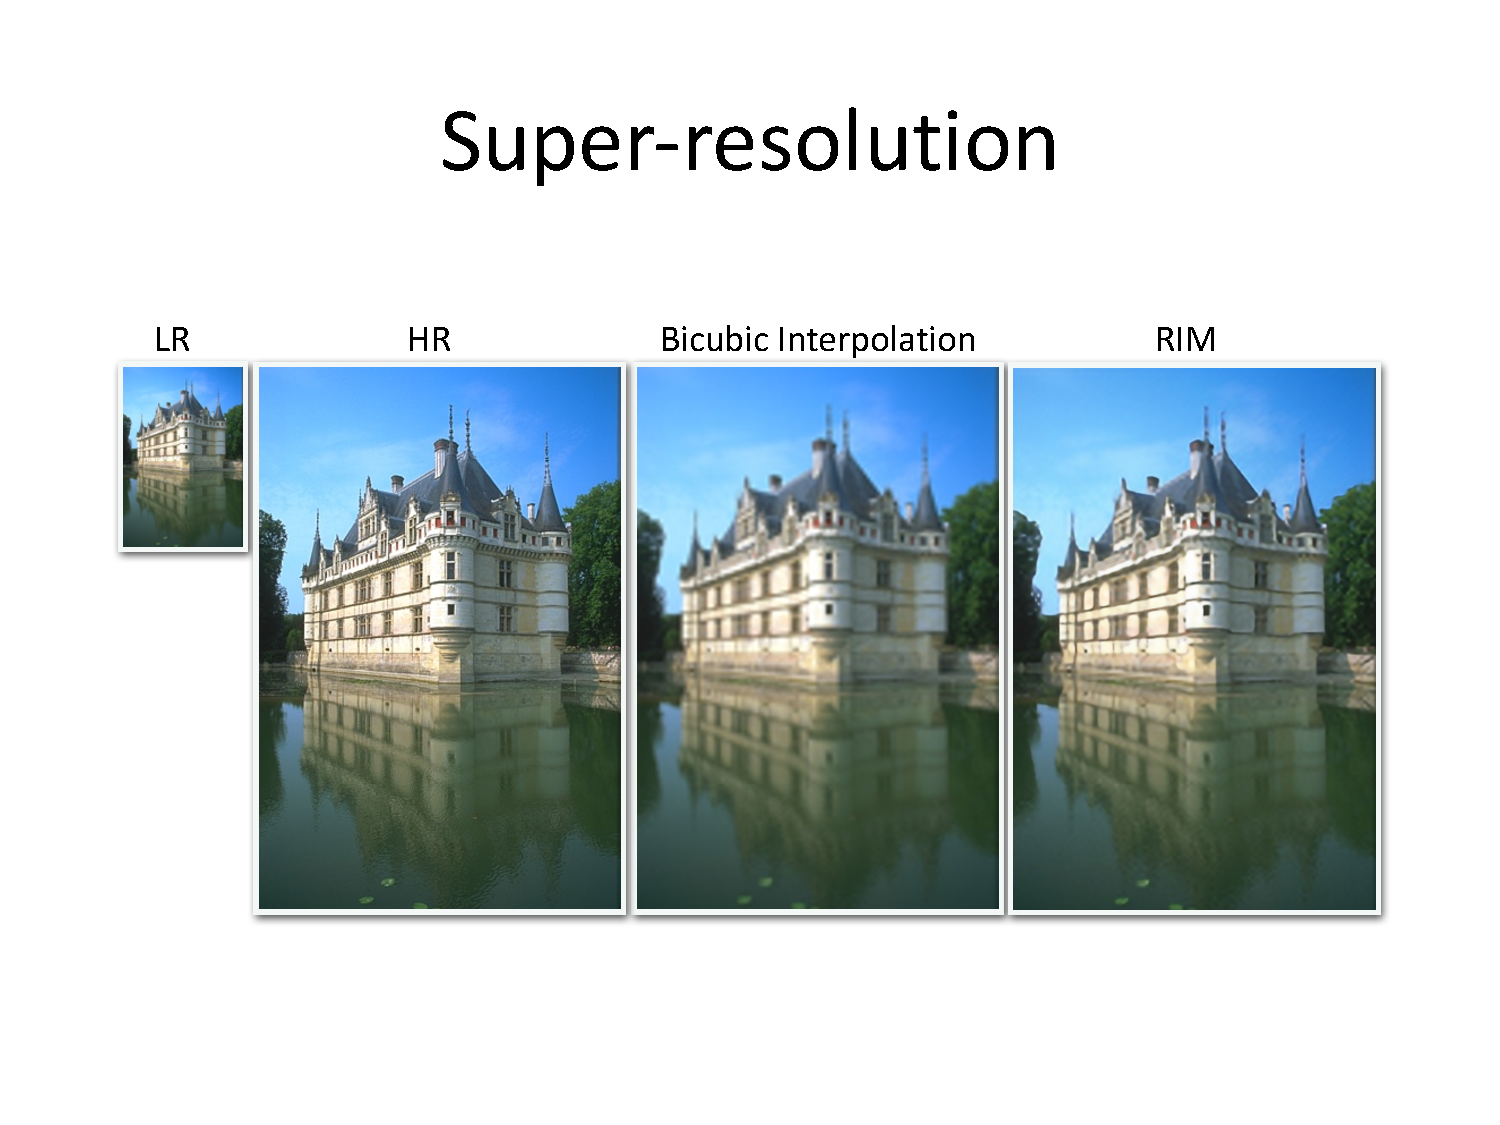
\includegraphics[width=0.86\textwidth]{super_resolution}
\end{frame}

\begin{frame}
    \frametitle{NIPS 2017: Deep Learning for Physical Sciences (3/4)}
    \bluelink{%
        https://dl4physicalsciences.github.io/files/nips_dlps_2017_slides_welling.pdf%
    }{%
        Unrolling Inference: For Astronomy and MRI Imaging%
    } \citep{WellingNIPS17} \\[1ex]

    \centering
    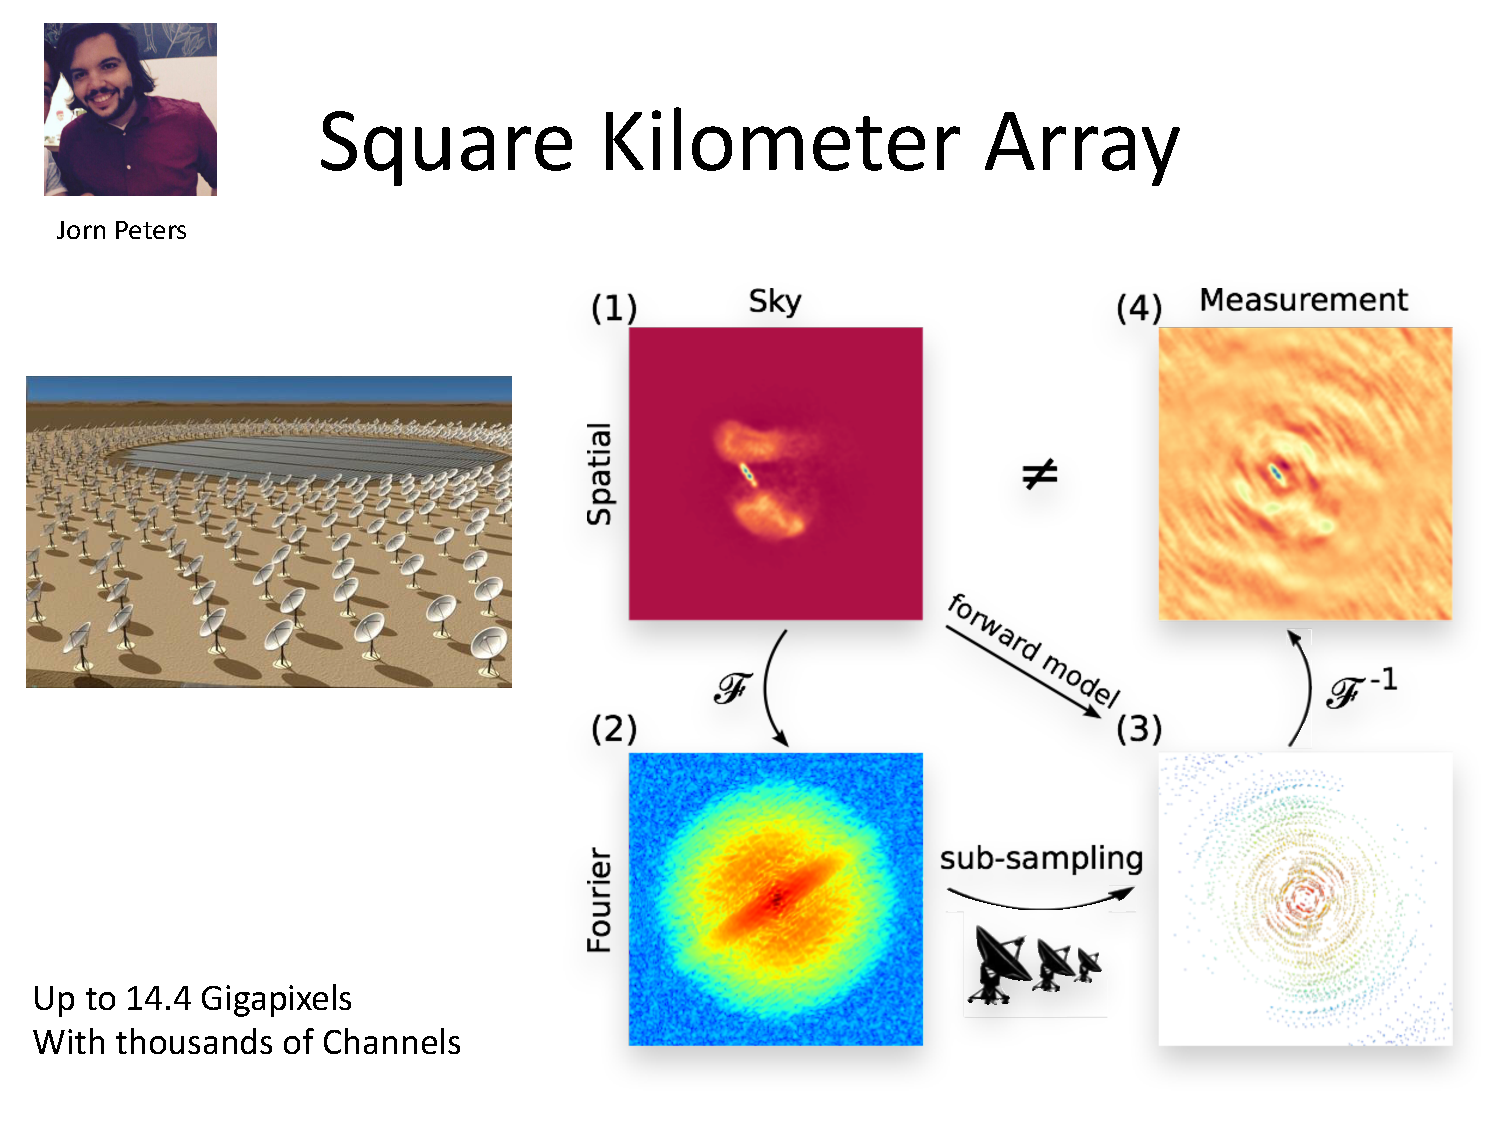
\includegraphics[width=0.86\textwidth]{radio}
\end{frame}

\begin{frame}
    \frametitle{NIPS 2017: Deep Learning for Physical Sciences (4/4)}
    \bluelink{%
        https://dl4physicalsciences.github.io/files/nips_dlps_2017_slides_karpatne.pdf%
    }{%
        How Can Physics Inform Deep Learning Methods in Scientific Problems: Recent Progress and Future Prospects%
    } \citep{KarpatneNIPS17} \\[1ex]
    \begin{itemize}
        \item Good concise high-level overview of ML \& physics; check it out!
    \end{itemize}

    \centering
    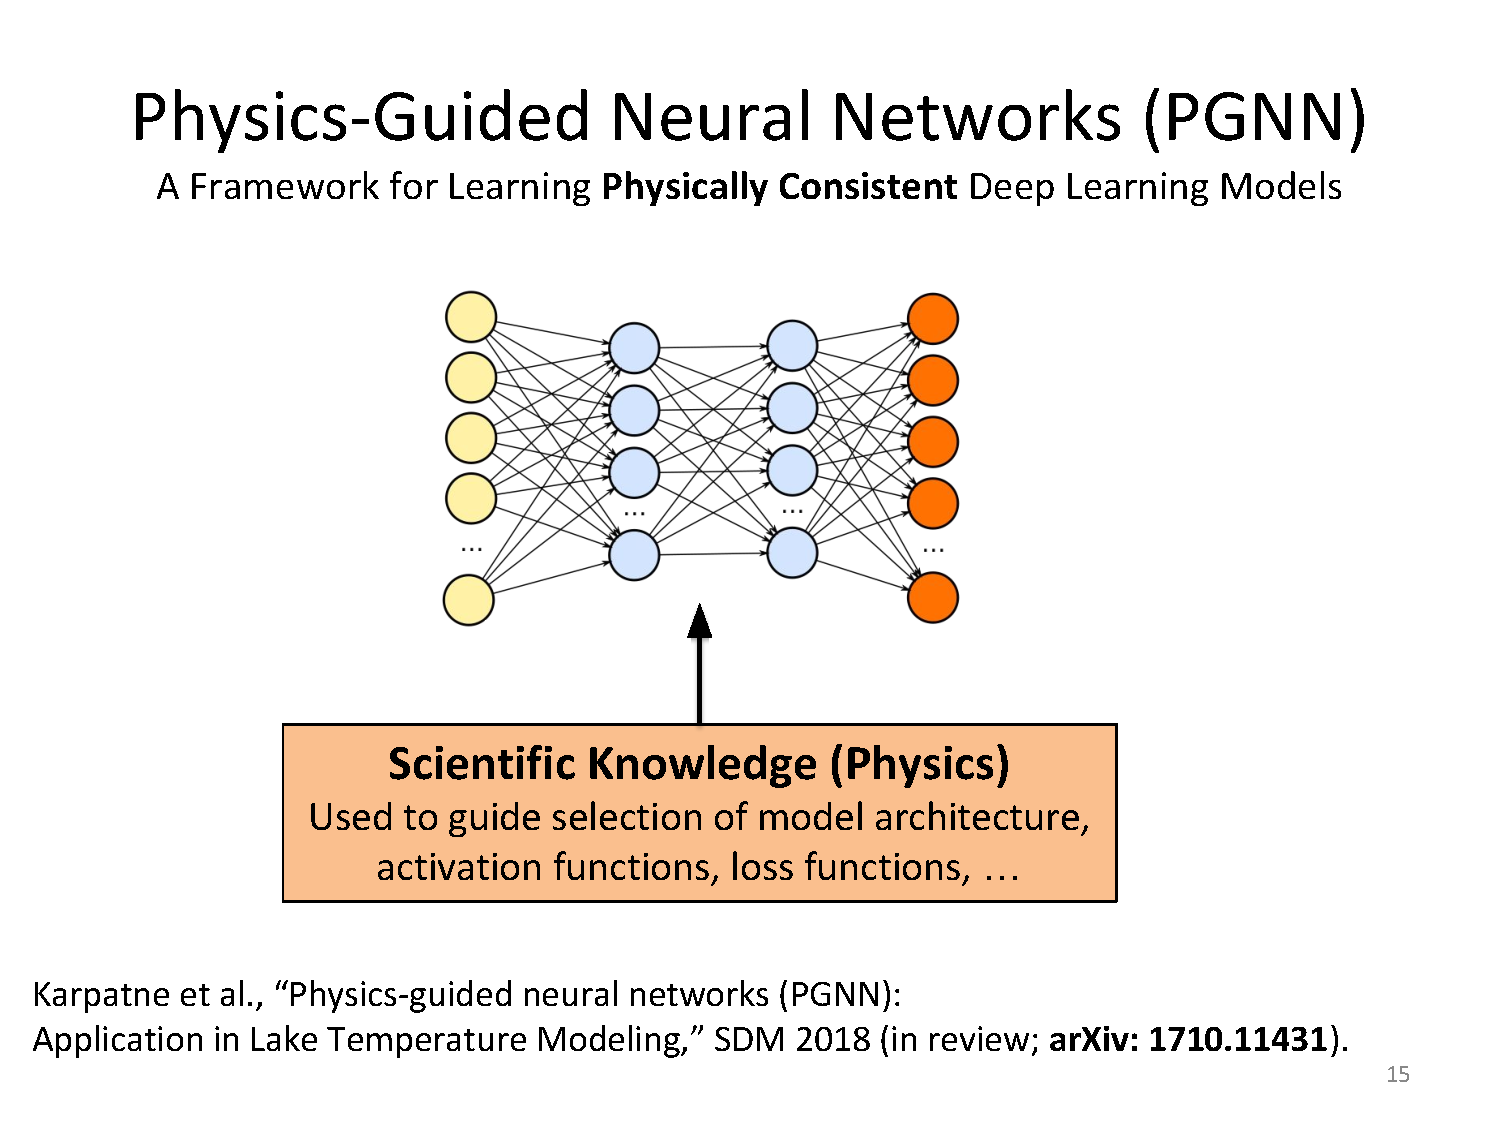
\includegraphics[width=0.77\textwidth]{pgnn}
\end{frame}

\begin{frame}
    \frametitle{Machine learning in fluid dynamics: APS DFD 2017}
    Some examples:
    \begin{itemize}
        \item Local Learning Strategies for Wake Identification (USC)
        \item Learning to classify wakes from local sensory information (USC)
        \item Drag Reduction of an Airfoil Using Deep Learning (UC Berkeley)
        \item Characterization and prediction of extreme events in turbulence (NYU/Courant)
        \item Machine Learning-based discovery of closures for reduced models of dynamical systems (U Michigan Ann Arbor)
        \item A Deep Learning based Approach to Reduced Order Modeling of Fluids using LSTM Neural Networks (OSU)
        \item Data-driven discovery of Koopman eigenfunctions using deep learning (UW)
    \end{itemize}
\end{frame}

\begin{frame}
    \frametitle{My advice}

    \begin{itemize}
        \item Pursue ML research in fluids
        \item Or don't, but pay close attention to what others are doing.
        An ML explosion in fluids might or might not happen; if it does, don't miss it.
    \end{itemize}
    \pause

    \begin{block}{What do fluid dynamicists need to do right now?}
        \begin{itemize}
            \item 40\% of the work: catch up to the rest of world on ML
            \item 50\%: figure out \alert{what the right problems are} in the first place
            \item Remaining 10\%: solve them
        \end{itemize}
    \end{block}
    \pause

    Be warned: the ML research community is \emph{extremely} fast-paced
    \begin{itemize}
        \item Most cited papers seem to be $< 2$ years old
        \item Anything older is likely obsolete!
        \item Common for previously unsolved problems to be solved within months; must keep up with conferences \& arXiv
    \end{itemize}
\end{frame}

\begin{frame}
    \frametitle{My objective}

    \begin{itemize}
        \item<+-> Teach a semester's worth of machine learning material in two hours
        \begin{itemize}
            \item Except for \emph{recurrent neural networks}: they're particularly relevant for dynamical systems, so we'll spend two hours on that Thursday
        \end{itemize}
        \item<.-> Obviously I can't go into much detail about anything
        \item<+-> You guide the next two hours:
        \begin{itemize}
            \item Stop me and ask lots of questions if you want \smiley
            \item Or just let me talk, either way
        \end{itemize}
        \item<+-> I will use standard ML terminology/notation, instead of tailoring to an engineering audience
        \begin{itemize}
            \item Otherwise you won't be able to understand the ML literature
        \end{itemize}
    \end{itemize}
\end{frame}

\begin{frame}
    \frametitle{What I will not do}
    \begin{itemize}
        \item<+-> Offer expert knowledge on machine learning in fluids/engineering/physics
        \begin{itemize}
            \item That's because I'm not an expert on that
        \end{itemize}
        \item<+-> Teach how to write ML code
        \begin{itemize}
            \item That would require its own lecture
            \item Today and Thursday will be mostly theory, with some brief examples
            \item $\exists$ some links to example code in today's \& Thursday's slides
        \end{itemize}
    \end{itemize}
\end{frame}

%%% Local Variables:
%%% mode: latex
%%% TeX-master: "../nn"
%%% End:
